% -------------------- DON'T EDIT ----------------------------------------
\documentclass[a4paper,12pt,oneside,openany]{xepersian-thesis-znu-ftex}
\usepackage[top=3.5cm,right=3cm,bottom=4cm,left=3cm]{geometry}  
\usepackage{amsmath}
 \usepackage[marginal,stable,bottom]{footmisc}     % for footnotes: marginal --> the same margins as text, 
                                                                                  %                       stable--> ?
                                                                                  %                       bottom --> starting the footnotes at a fixed place at the bottom of the page.
 
\usepackage{perpage}                                             % for footnotes: starting from 1 perpage
\MakePerPage{footnote}
\usepackage{cite}                                                     % for collecting citations: [1,2,3,4] --> [1-4]
\usepackage{setspace}                                            % for switching between double/single space in document
\allowdisplaybreaks                                                    % breaking the lines&pages when needed for the style.
\usepackage{parskip}                                               % ? 

%\relpenalty=9999                                            % show the neccessity of breaks for lines, changing the number to 10000 cause no break in lines.
%\binoppenalty=9999

\usepackage{xecolor}
\usepackage{amsmath}
\usepackage{makeidx}
\usepackage{verbatim}
\usepackage[colorlinks,linkcolor=blue,citecolor=blue]{hyperref}
\usepackage{graphicx}
\usepackage{ifthen}

 
% ‎‏برای‎ ایجاد فاصله در اول هر پاراگراف از دستور زیر استفاده می‌نماییم‏، باید دقت کنیم که یک پاراگراف با دو اینتر بعد از پاراگراف قبل ایجاد می‌شود و استفاده از // به معنای ایجاد پاراگراف بعدی نیست.
\setlength{\parindent}{20pt}


\makeatletter
\pdfstringdefDisableCommands{%
\let\lr\@firstofone
}
\makeatother
% ----------------------------------------------------------------------------
\usepackage{xepersian}

\usepackage[Lenny]{fncychap}

\settextfont[Scale=1.07]{XB Niloofar}
\setlatintextfont[Scale=1.05]{Times New Roman} 
\setdigitfont[Scale=1.05]{Yas} 
% قلم برای اعداد به صورت فارسی با صفر توخالی، در صورتی که بخواهیم اعداد انگلیسی نوشته شوند این خط را غیر فعال می‌کنیم.

\defpersianfont\nastaliq[Scale=2.0]{IranNastaliq}
% قلم برای نوشتن تقدیم
\defpersianfont\nastaliqone[Scale=1.0]{IranNastaliq}
% قلم نستعلیق با سایز متناسب با متن در صورت نیاز
\defpersianfont\anotherfont[Scale=1.2]{B Zar}
% قلم برای نوشتن تشکر (قلم فانتزی)
\newenvironment{fantezi}
{\anotherfont }


\makeindex


\def\beginto{
\newpage
\begin{RTL}
\begin{Huge}
\nastaliq

\begin{center}
\vspace*{0.15cm}
تقدیم به 
}

\def\endto{
~
\end{center}
\end{Huge}
\end{RTL}
}

\def\beginthanks{
\newpage

{\centering\Huge{\nastaliqone{
تشکر وقدردانی ~\\
~\\}}}
}

\def\endthanks{
~
}

\def\thanks{
\beginthanks
در اینجا از همه کسانی که در این سال ها به من کمک  کرده اند تشکر  می کنم. 



\endthanks
}

\def\startpage{
\newpage
\pagenumbering{gobble}
\vspace*{3cm}
\begin{center}

\includegraphics[width=12cm]{besm}
\end{center}
}
\makeatletter
\def\@makechapterhead#1{%
  \vspace*{50\p@}%
  {\parindent \z@ \centering\normalfont
    \ifnum \c@secnumdepth >\m@ne
      \if@mainmatter
        \huge\bfseries \@chapapp\space \tartibi{chapter} 
        \par\nobreak
        \vskip 20\p@
      \fi
    \fi
    \interlinepenalty\@M
    \Huge \bfseries #1\par\nobreak
    \vskip 40\p@
  }}
\def\@makeschapterhead#1{%
  \vspace*{50\p@}%
  {\parindent \z@ \centering
    \normalfont
    \interlinepenalty\@M
    \Huge \bfseries  #1\par\nobreak
    \vskip 40\p@
  }}
\makeatother



\renewcommand\bibname{مراجع}
\def\contentsname{فهرست}

% some extra diffinitions %%%%%%%%%%%%%%%%%
%%%%%%%%%%%%%%%%%%%%%%%%%%%%%

\def\bea{\begin{eqnarray}}
\def\eea{\end{eqnarray}}

\def\ba{\begin{array}}
\def\ea{\end{array}}

\def\ni{\noindent}
\def\nn{\nonumber}

\def\bc{\begin{center}}
\def\ec{\end{center}}


% ------------------- You Can EDIT ----------------------------------------
% The paths to the images.
\graphicspath{{chap1_images/}{chap2_images/}}                       

% -------------------- DON'T EDIT ----------------------------------------
\begin{document}
% -------------------- PLEASE EDIT ---------------------------------------

% --------------------------------------   INFORMATION IN PERSIAN  ---------------------------------------

\title{پایان‌نامه من با زی‌پرشین}
\author{نام نام خانوادگی}
%--------------------------------------------
\degree{کارشناسی}
%---------------------------------------------
\supervisor{نام استاد راهنما}
% در صورتی که استاد مشاور داشته‌اید نام وی را در خط زیر بنویسید در غیر این صورت خط زیر باید غیرفعال باشد.
%\advisor{نام استاد مشاور} \advisorexisttrue
\department{کامپیوتر}
\university{دانشگاه زنجان}
\city{زنجان}
\thesisdate{\today}
\makepersiantitle
% -------------------------------------------------------------------------------------------------------------------
\startpage
% -------------------------------------------------------------------------------------------------------------------

\beginto
%%در اینجا پایان‌نامه خود را به هر کس که دوست دارید تقدیم کنید. در غیر این صورت این قسمت را غیر فعال کنید.
...
\endto
% -------------------------------------------------------------------------------------------------------------------
%اگر در فایل thanks از دوستان و همکاران خود تشکر کرده‌اید خط زیر را فعال کنید، در غیر این صورت این خط باید غیرفعال باشد.
\thanks
% -------------------------------------------------------------------------------------------------------------------
\newpage
\begin{abstract}
% To add the abstract in the index.
\addcontentsline{toc}{section}{چکیده} 
چکیدهٔ پایان‌نامه خود را به زبان فارسی در این قسمت بنویسید.
\keywords{کلمهٔ کلیدی اول، کلمهٔ کلیدی دوم، کلمهٔ کلیدی سوم}
\end{abstract}
% -------------------------------------------------------------------------------------------------------------------
% اضافه کردن فهرست محتوا - شکل - جدول
\tableofcontents
\listoffigures
\listoftables
% -------------------------------------------------------------------------------------------------------------------

% اگر قبل از شروع فصل‌های پایان‌نامه مقدمه‌ای دارید، خط زیر را فعال کرده و مقدمه خود را در فایل introduction بنویسید. در غیر این صورت این خط باید غیر فعال باشد.
\newpage
\pagenumbering{arabic}\setcounter{page}{1}
\newpage
\vspace*{-1cm}
\section*{پیش‌گفتار}
\addcontentsline{toc}{section}{پیش‌گفتار}
در اینجا اگر دوست داشتید چند پاراگرافی را به عنوان پیش‌گفتار پایان‌نامه بنویسید.

% ----------------------------------------   Chapters of the Thesis  ---------------------------------------------
% if any un-wanted empty page is produced between chapters, you can use \input instead of \include : \chapter{عنوان فصل یا پیوست}
متن فصل را در اینجا بنویسید.

\section{عنوان بخش }
متن بخش اول را در اینجا بنویسید.
% نحوه اضافه کردن تصویر با ظاهر در همان نقطه‌ای که قرار گرفته است.
\begin{figure}[H]
% تگ H باعث می‌شود تصویر را در همان مکانی که اضافه کردید قرار بگیرد.
\centering
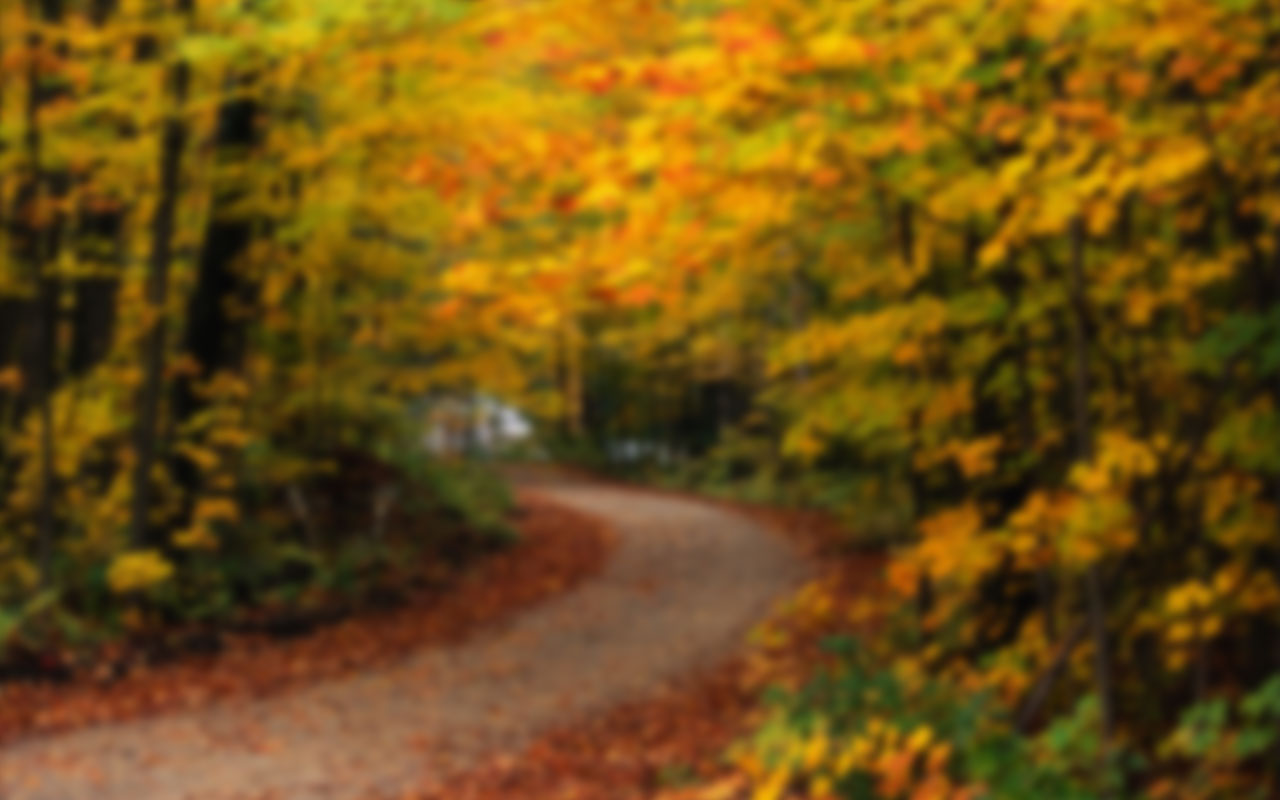
\includegraphics[scale=0.3]{chap1_images/sample.jpg}
\caption[c_1]{c_2}
% c_1 : عنوان تصویر در فهرست
% c_2 : عنوان تصویر در متن، مرجع را نیز در این قسمت ذکر کنید
\label{sample}
% برای ارجاع دادن در متن استفاده می‌شود.
\end{figure}

\subsection{عنوان زیر بخش }
متن زیر بخش اول را در اینجا بنویسید.

\chapter{عنوان فصل یا پیوست}
متن فصل را در اینجا بنویسید.

\section{عنوان بخش }
متن بخش اول را در اینجا بنویسید.
% نحوه اضافه کردن تصویر با ظاهر در همان نقطه‌ای که قرار گرفته است.
\begin{figure}[H]
% تگ H باعث می‌شود تصویر را در همان مکانی که اضافه کردید قرار بگیرد.
\centering
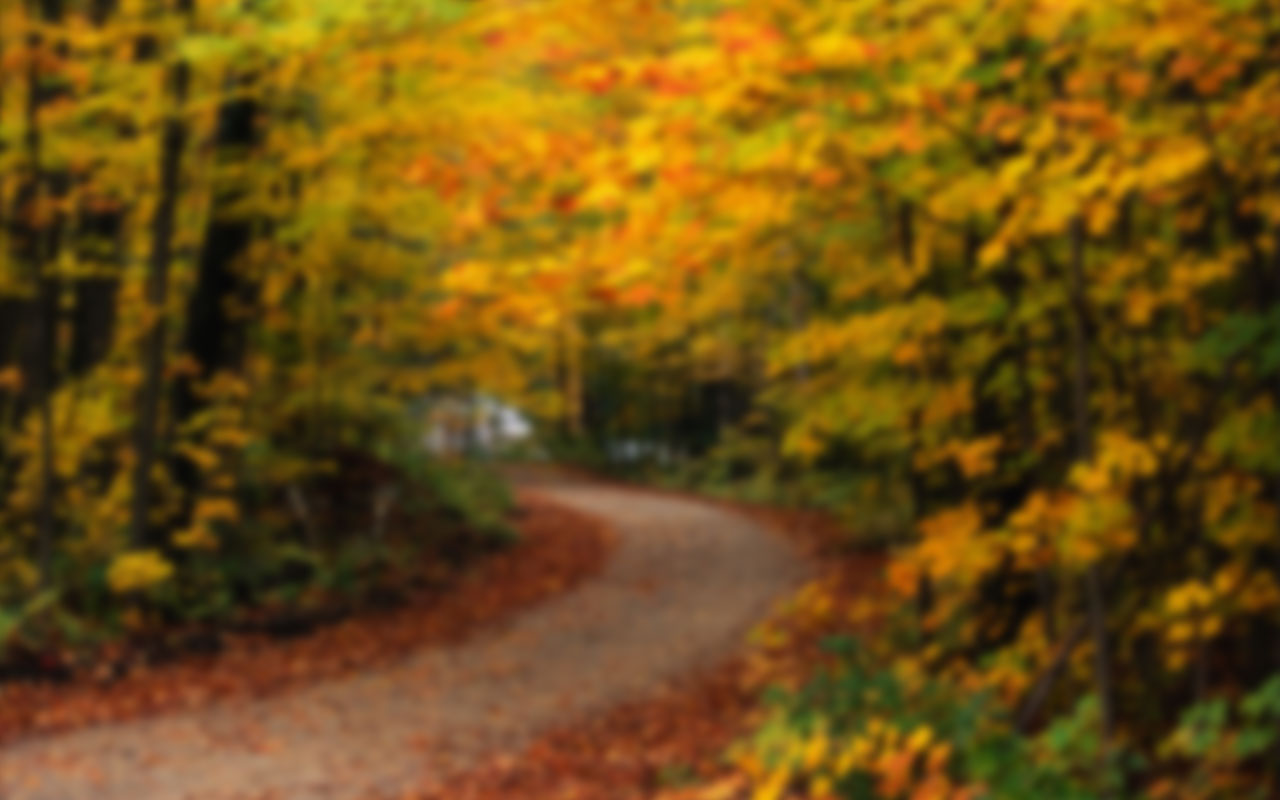
\includegraphics[scale=0.3]{chap1_images/sample.jpg}
\caption[c_1]{c_2}
% c_1 : عنوان تصویر در فهرست
% c_2 : عنوان تصویر در متن، مرجع را نیز در این قسمت ذکر کنید
\label{sample}
% برای ارجاع دادن در متن استفاده می‌شود.
\end{figure}

\subsection{عنوان زیر بخش }
متن زیر بخش اول را در اینجا بنویسید.
 
\chapter{عنوان فصل یا پیوست}
متن فصل را در اینجا بنویسید.

\section{عنوان بخش }
متن بخش را می توانید در این ناحیه بنویسید.

\subsection{عنوان زیر بخش }
متن زیر بخش را می توانید در این قسمت بنویسید
\chapter{عنوان فصل یا پیوست}
متن فصل را در اینجا بنویسید.

\section{عنوان بخش }
متن بخش را می توانید در این ناحیه بنویسید.

\subsection{عنوان زیر بخش }
متن زیر بخش را می توانید در این قسمت بنویسید
\chapter{عنوان فصل یا پیوست}
متن فصل را در اینجا بنویسید.

\section{عنوان بخش }
متن بخش را می توانید در این ناحیه بنویسید.

\subsection{عنوان زیر بخش }
متن زیر بخش را می توانید در این قسمت بنویسید

%--------------------------------------------------------------------------------------------------------
% -------------------- DON'T EDIT ----------------------------------------
% the following lines are needed for making the appendixes name correct in the index.
\makeatletter
\def\@makechapterhead#1{%
  \vspace*{50\p@}%
  {\parindent \z@ \centering\normalfont
    \ifnum \c@secnumdepth >\m@ne
      \if@mainmatter
        \huge\bfseries \@chapapp\space \thechapter
        \par\nobreak
        \vskip 20\p@
      \fi
    \fi
    \interlinepenalty\@M
    \Huge \bfseries #1\par\nobreak
    \vskip 40\p@  }}
%--------------------------------------------------------------------------------------------------------
% -------------------- Please EDIT ----------------------------------------

\appendix
\chapter{عنوان فصل یا پیوست}
متن فصل را در اینجا بنویسید.

\section{عنوان بخش }
متن بخش را می توانید در این ناحیه بنویسید.

\subsection{عنوان زیر بخش }
متن زیر بخش را می توانید در این قسمت بنویسید 
\chapter{عنوان فصل یا پیوست}
متن فصل را در اینجا بنویسید.

\section{عنوان بخش }
متن بخش را می توانید در این ناحیه بنویسید.

\subsection{عنوان زیر بخش }
متن زیر بخش را می توانید در این قسمت بنویسید

\bibliographystyle{unsrt-fa}
% اگر فایل bibtex با پسوند bib حاوی اطلاعات مربوط به مراجع خود با فرمت صحیح bibtex را دارید از خط زیر استفاده کنید و به جای MyReferences نامه فایل خود را بنویسید.

% در این نمونه پایان‌نامه فرض شده است که شما فایل bib حاوی اطلاعات مربوط به مراجع خود با نام MyReferences.bib را دارید.
\bibliography{MyReferences}

% اگر به صورت عادی می‌خواهید ارجاع دهید خط بالا را غیر فعال کرده و قسمت زیر را فعال کنید و طبق مثال عمل کنید (البته این روش حرفه‌ای نیست و توصیه نمی‌شود).
% \begin{thebibliography}{99} % assumes less than 100 references
\addcontentsline{toc}{section}{مراجع} % to add the references to index
%چنانچه مرجع فارسی نیز داشته باشید باید دستور فوق را فعال کنید و مراجع فارسی خود را بعد از این دستور وارد کنید
\Persian
\bibitem{ali}
علی روستایی، مسعود پورموسی و فرشاد عبداللّه‌نیا \emph{کارگاه آموزشی زی‌پرشین}، دانشکده مهندسی مکانیک، دانشگاه صنعتی شریف، زمستان ۱۳۸۸

\Latin
\bibitem{wiki}
\url{http://en.wikipedia.org/wiki/DNA}

\end{thebibliography}


% include persian to english dictionary
   %
   % در صورتی که می‌خواهید عنوان «واژه‌نامه فارسی به انگلیسی» در فهرست مطالب 
   % وارد شود، علامت «%» را از ابتدای خط زیر حذف کنید.
\addcontentsline{toc}{section}{واژه‌نامه فارسی به انگلیسی }

\begin{center}
\vspace{1.5cm}
\Huge{واژه‌نامه فارسی به انگلیسی}
\vspace{1.5cm}
\end{center}
%\begin{center}
%الف
%\end{center}
آدنین                              \dotfill               \lr{adenine}                       \\
اتصال                              \dotfill               \lr{binding}                       \\
اتصال‌گر                           \dotfill               \lr{linker}                       \\

%\begin{center}
%ب
%end{center}
باز                                \dotfill               \lr{base}                       \\
بازپیچیده                         \dotfill               \lr{over-twist}                     \\
باز نیتروژنی                      \dotfill               \lr{nitrogenous base}                       \\
بالادست                            \dotfill               \lr{upstream}                            \\
بیان ژن                           \dotfill               \lr{gene expression}                       \\

%\begin{center}
%پ
%\end{center}
پای پیچ                           \dotfill               \lr{pitch}                         \\
پلیمریزاسیون                      \dotfill               \lr{polymerisation}                      \\
پیش‌برنده                          \dotfill               \lr{promoter}                        \\

% و به همین ترتیب می‌توانید ادامه دهید.
 

% --------------------------------------   INFORMATION IN LATIN  ----------------------------------------------
\begin{latin}
\latintitle{My Thesis in XePersian}
\latinauthor{First Name Last Name}
% --------------------------------------
% choose and activate one of the following lines
\latindegree{Bachelor's Thesis}
% --------------------------------------
\latinthesisdate{\latintoday}
\latinsupervisor{Name of Supervisor}
% If you have advisor, write its name in the following line, otherwise inactive (comment) the line.
%\latinadvisor{Name of Advisor} \advisorexisttrue
\latindepartment{Computer Science}
\latinuniversity{University of Zanjan}
\latincity{Zanjan}
\begin{latinabstract}
\noindent 


\latinkeywords{Keyword1, Keyword2, Keyword3}

\end{latinabstract}
\makelatintitle
\end{latin}

\end{document}
